
\documentclass[a4paper, 11pt, english, twoside, openright]{article}
  %\documentclass[a4paper,10pt]{scrartcl}
\ProvidesPackage{mystyles}
 \usepackage[utf8]{inputenc}
\usepackage[sort]{natbib}
\usepackage{amsmath}
  \usepackage{authblk}
\usepackage[version=3]{mhchem}
\usepackage{graphicx}
\usepackage{url}
\usepackage{babel,textcomp} 
\usepackage{listings}
\setcounter{secnumdepth}{2}
\setcounter{tocdepth}{2}
\usepackage{caption}
\usepackage{subcaption}
\usepackage{amssymb}
\usepackage[normalem]{ulem} %for strikeout
\usepackage{pdfpages} %to include pdf document
\usepackage[toc,page]{appendix} %for appendix environment
%\setlength{\parindent}{15pt}
\usepackage{float}
\restylefloat{figure}
\usepackage{wrapfig}

%\pretolerance = 2000
%\tolerance = 5000   
%\hbadness = \tolerance

\usepackage{booktabs}
%\usepackage{arydshln}
\usepackage{longtable}
\usepackage{changepage}
\usepackage{float}
\usepackage[hidelinks]{hyperref}
\newcommand\B{\rule[-1.2ex]{0pt}{0pt}}
\renewcommand{\arraystretch}{1.2} 
\usepackage{float}
\restylefloat{table}
%\usepackage{deluxetable}
%\usepackage[]{mcode}
\usepackage{rotating}
\usepackage[margin=1in]{geometry}
\usepackage[tableposition=top]{caption}
  

\title{Experimental investigation of solitary breaking waves in the swash zone. }
\author[1]{Lisa Smith}	
\author[1]{Atle Jensen}
\author[1]{Geir Pedersen}

\affil[1]{ Department of Mathematics, University of Oslo, Norway}
	% Activate to display a given date or no date
\begin{document}
\maketitle


\begin{abstract}
This study presents an experimental investigation of plunging breakers on a sloping beach with an inclination of $5.1^{\circ}$. The incident waves are solitary waves with various amplitudes from non-breaking waves to plunging breakers, and the area investigated is the swash zone. PIV (Particle Image Velocimetry) is performed on images captured at four different field of views (FOV). The PIV measurements are compared with computed velocity fields from a Boundary Integral Model (BIM). 
There is excellent agreement between the experimental and the computed result for the non-breaking waves. The experimental results from the breaking waves indicate that the motion becomes more irregular as we move further up the beach. In addition, there seem to be more irregularities present  for waves with larger amplitude. Shoreline position and maximum runup are measured, and are repeatable in both time and height, although  cross-sectional variations of the shoreline shape are observed at maximum runup.  Length and velocity of air bubbles entrapped by the plunger breakers are extracted from a image series captured with large a FOV. The images showed that a large air bubble seems to be stable for a time period during runup for the breaking waves.
%Surface profiles of the runup were investigated at large scale and revealed that the surface of the breaking waves were unstable for a time period during uprush.
\end{abstract}

\section{Introduction}
In shallow water with constant depth, the nonlinear effect and dispersion will be balanced for solitary waves \citep{peregrine1983breaking}. If the depth decreases as the wave travels towards the shore, the wave will steepen, and at some critical  point breaking may occur. Breaking waves are one of the most important physical features in the swash zone \citep{elfrink2002hydrodynamics}. Breaking waves have a large impact on sediment transport onshore, which can result in erosion on cliffs and affect construction located near the shore. Although breaking waves is a well-known phenomenon from our daily life, many physical aspects regarding wave breaking are still poorly understood.

%Both computational and experimental methods have difficulties predicting tafter the wave breaking.

%Experimental work on solitary breaking wave have



 %Currently no analytical theory is able to predict the post stages of wave breaking.


 Several experimental studies of breaking waves have been performed in the recent years. A broad range of different experimental methods have been utilized to measure quantities such as surface elevation, runup, shear stress, and velocities. Techniques such as Laser Doppler Velocimetry \citep{petti01}, PIV \citep{cowen03} and shear sensors \citep{Barnes09}  has been utilized. The swash zone is defined as the region where the beach is partly wetted during runup and rundown. Aeration and the 
small flow depth makes the swash zone a challenging region to study experimentally with the techniques mentioned above. A further development of the PIV method is Bubble image Velocimetry (BIV), which \cite{rivillas2012estimation} use to investigate velocity fields in plunging breakers.\marginpar{\footnotesize What did they find ?}
 
 
 % \cite{pujara2015experimental} investigated the flow evolution of the runup and run down of breaking solitary waves, in additon to 
 
 

 
%The swash zone is defined as the region where the beach is partly wetted during runup and run down.
 
%\cite{jensen2003experimental} performed an experimental investigation of wave run-up at a steep beach, where Particle Image Velocimetry (PIV) was performed when the wave front was at its steepest. They compared the measurements with a Boussinesq model. The beach slope was $10.54^\circ$ and they found that the waves with the largest amplitude was close to breaking, since a part of the wave front almost formed a plunging jet.

%\cite{petti01} did turbulence experiments of plunging and collapsing breakers. The experiments were carried out in a 48m long and 0.8m wide flume. They used  Laser Doppler Velocimetry (LDV) to measure instantaneous velocities. The velocities were measured 0.5mm above the beach bed. They concluded that turbulent energy is higher during up-rush than backwash. %They found that kolomogorov micro length scale had it maximum at the bottom of the bed. The length scale decreased towards the free surface. This is the opposite of the characteristic of plane channel flow with a free surface. 

%\citep{cowen03} used PIV with fluorescent particles to investigate the swash zone. The fluorescent particles enabled them to investigate areas where the flow was affected by air bubbles. They generated both spilling and plunging breakers with a period T=2.0s. They found that the up-rush turbulence was dominated by the bore, while the backwash was dominated by wall bounded turbulence. The experiment was conducted in a 32m long and 0.6m wide wave tank, with a beach slope with an inclination of 1:20. %The shear stress was calculated from the friction velocity, which depends on the dissipation, von karman constant and distanse to the wall.%There seems to be tendency that the up-rush friction coefficient is larger than the backwash coefficients. 

%A large and medium scale measurement of bed shear stress in bore driven swash was conducted by \cite{Barnes09}. They used a shear plate, based on a shear cell developed by \cite{grass1995shear}. The surface of the shear plate was smooth and with dimensions 10cm x 20cm. The medium scale experiment was done in a 20m long and 0.45m wide flume. The slope was 1:10 and two different grades of roughness were employed at the beach. The large scale experiment was done in a 20m long and 0.85m wide flume. Experiments were done with different roughness and the beach had a slope of 1:12.   The results revealed that the bed shear stress had its maximum value at the bore arrival and then decreased with time. The backwash maximum was about 2-4 times less than the up-rush maximum, which is in accordance to \cite{cowen03}. 

% \cite{kikkert11} did measurements on a bore driven swash. The experiments were carried out in a 20m long flume with a width of 0.45m. They used PIV to measure velocities and Laser-Induced Fluorescence (LIF) to measure the water depth. The beach slope was 1:10 and the experiments were repeated on beaches with different roughness. This study concludes that the up-rush friction factors are smaller than friction factors for backwash. This contradicts the findings from the work done by \cite{cowen03} and \cite{Barnes09}. \cite{rivillas2012estimation} used Bubble image Velocimetry (BIV) to investigate velocity fields in the swash and surf zone for plunging breakers. A numerical model based on Reynolds Average Navier Stokes (RANS) equation was used to compare the measurements. \cite{rivillas2012estimation} found that the BIV measurements were in agreement with the RANS model. 

Until now, PIV measurements with high resolution close to the beach have not been reported for breaking waves in the swash zone. This paper presents PIV measurements where the amplitude of the solitary breaking waves varies. The paper starts with a description of the experimental set-up in chapter \ref{experimnetal-set-up}. Further on, results from different parts of the experiment will be presented, herein the surface elevation of the incident waves in chapter \ref{surf_elev}, surface development and maximum runup in chapter\ref{max_run}, velocity profiles from the swash zone in chapter \ref{vel_pro}, and air bubble investigation in chapter \ref{bub_inv}. Finally, a discussion of the findings will be present in the last chapter \ref{con_rem}.

\section{Experimental set-up and formulation}
\label{experimnetal-set-up}

\subsection{The wave tank}
Laboratory experiments of non-breaking to plunging breaking waves in the swash zone were conducted in  a 25m long and 0.51m wide wave tank 
located at the Hydrodynamics Laboratory at the University of Oslo.
Incident waves were generated in an equilibrium depth of $20.5$cm by
a piston type wave paddle using the method described in 
\cite{jensen2003experimental}. 
A PETG (Polyethylene Terephthalate Glycol-modified) beach with an inclination of $5.1^{\circ}$ was placed in the wave tank with its toe 529.81cm from the start position of the wave paddle.   Two coordinate systems were introduced, one parallel to the still water level $(x',z')$, and one parallel to the beach $(x,z)$ (See Figure \ref{fig:beach_tegning}).  The origin of both is at the equilibrium shoreline.

Nominally, the amplitude to depth ratios, $A/H$, should equal (0.1,0.2,0.3,0.4,0.5).  
However, imperfection in the generation and frictional effects along
the wave tank reduced the heights slightly.  
An acoustic wave gauge (ultra Banner U-Gage S18U, sample frequency of 200Hz) measured the wave height at the toe of the beach. After correcting for reflections (see ...) the amplitudes were found to be
  $A/H=(0.0989, 0.1191, 0.1981, 0.2958, 0.3939, 0.4874)$.\marginpar{\footnotesize Are the amplitudes corrected ? The way this correction is made must be described.}


\begin{figure}[]
\centering
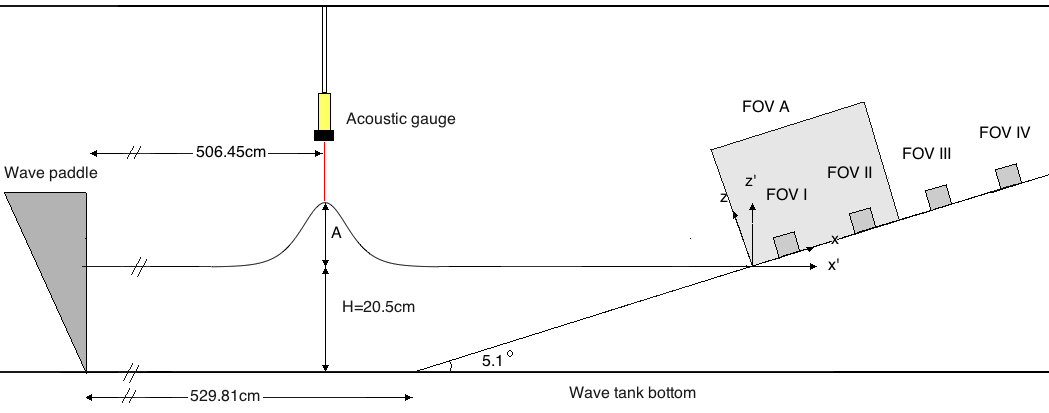
\includegraphics[width=\textwidth]{./Figures/setup3.png}
%http://commons.wikimedia.org/wiki/File:Breaking_wave_types.gif
\caption{\textit{ Sketch of  the experimental set-up.}}
\label{fig:beach_tegning}
\end{figure}

\subsection{Instrumentation, measurements}
To obtain velocity fields in the swash zone, images were captured at four different field of views (FOV), located upward along the beach (Table \ref{tab:loc}). The different FOV's are denoted with roman numbers. The water in the tank was seeded with polymid particles with diameters of approximately 50 $\mu$m. A Quantronix Darwin Duo pulsed laser generated a light sheet parallel to the centreline of the wave tank, and a Photron SA5 high speed camera (1024 x 1024) synchronized with the laser, captured images of the illuminated particles. A Carl Zeiss Makro- Planer 2/50 zf lens was used. Images were collected at 3000 frames per seconds (fps).
 \begin{table}[]
 \centering
\caption{\textit{Location of the different FOVs  in $cm$. The dimensions of the FOVs are approximately 4cm x 4cm.}}
\begin{tabular}{|c|c|c|c|c|c|c|}
\hline
\textbf{FOV:}      & I                   & II                 & III     & IV \\ \hline
\textbf{Location, x:}& {[}8.49 - 13.04{]} & {[}36.35 - 40.26{]} & {[}77.55 - 81.53{]} & {[}117.76 - 121.80{]} 
 \\ \hline
\textbf{Location, z:}&  {[}-0.05 - 3.78{]} & {[}-0.16 - 3.54{]} & {[}-0.04 - 3.79{]} & {[}-0.85 - 3.09{]} 
\\ \hline
\end{tabular}
\label{tab:loc}
\end{table}
The image processing were performed in DigiFlow \citep{digiflow}. PIV was performed using interrogation windows of 32 x 8 pixels with a 75\% overlap. Oblong interrogation windows are beneficial in boundary layer flow and have been employed previously in \cite{Liu...} and \cite{pedersen2013runup}. An averaging in time was applied where 10 images was used.\marginpar{\footnotesize Are the averaging always 10?}

To investigate air bubbles encapsulated by the plunging breakers, the camera was moved further away from the wave tank, resulting in much larger FOV than the FOVs installed to obtain velocity fields. This FOV will be referred to as FOV A and is located at $x=[0-60]$cm.  500 fps were used in this investigation, and a continuous dedolight 400D was used as illumination, replacing the laser. A white background sheet was attached to the side wall of  the wave tank and the water was dyed dark blue to increase the contrast in the images.

The maximum runup was measured by capturing images of the shoreline at its maximum position. A high speed Photron APX  camera was mounted on rails above the beach in the wave tank with same inclination as the beach. A high pulsed white light was used as illumination. The field of views were based on estimates of the runup height for each case. The camera captured 125 frames per second. The maximum shoreline profiles were tracked manually for each wave.


Each experiment was repeated at least three times.
The scatter $\delta_i$ for some measured quantity, $\sigma_i$, is then calculated as,
\begin{equation}
\delta_i=\frac{\sigma_i-\overline{\sigma}}{\overline{\sigma}}
\end{equation}
where $\overline{\sigma}$ is the mean over the  repetitions.

\subsection{The potential flow model}
The evolution of the waves during shoaling, as well as the runup for the smallest amplitude, were 
computed by a BIM (Boundary Integral Model) for fully nonlinear, inviscid flow.
This model breaks down when a plunger re-attaches with fluid or impacts the beach. Moreover, the
model  becomes
singular when the contact angle at the shoreline exeeds $90^\circ$  and the results also become unreliable
for contact angles slightly smaller.  More details are given in  \cite{pedersen2013runup}.\marginpar{\footnotesize Grid refinement?}    
\section{Results}
\label{result}

Visual inspection of the experiments revealed that the cases with normalized amplitude $A/H=0.0989$ and $A/H=0.1191$ did not break until the draw-down, while all the other cases developed into plunging breakers at or before the equilibrium shoreline. This is in compliance with numerical studies by \cite{grilli1997breaking}\marginpar{\fotnotesize cannot just say this, but mut give the breaking limit from Grilli et al}. The plunger breakers encapsulated large amounts of air, which resulted in air bubbles in the swash tongue of the breaking waves (Figure \ref{fig:boble_bevis}).

\begin{figure}[]
\centering
\scalebox{1}[-1]{\includegraphics[angle=180,width=0.7\textwidth]{./Figures/BUBBLE/new_jan_bilde_bub.eps}}
%http://commons.wikimedia.org/wiki/File:Breaking_wave_types.gif
\caption{\textit{Image of the swash tongue for $A/H=0.4874$. }}
\label{fig:boble_bevis}
\end{figure}

\subsection{Surface elevation of the incident waves}
\label{surf_elev}
The amplitude of the smallest amplitude wave is determined by
a simple correction scheme. First the maximum of the series from the 
acoustic gauge is used as solitary wave amplitude in the BIM model.
For the lowest wave this value is $\eta_m/H=....$.
When BIM data are extracted at the gauge position we then obtain 
a slightly too large surface elevation, due to the reflection from 
the beach, namely $\eta_b/H=...$. We then adjust the amplitude 
according to $A=\eta_m-(\eta_b-\eta_m)$. 
The result is $A/H=0.0989$ and the comparison with BIM results, obtained with this amplitude for the incident wave,
 is shown in Figure \ref{fig:surf_ele1}. Cubic polynomial regression is used to remove noise from the signal, and linear interpolation is used to fill 
in  dropouts. The surface elevation measurements are in agreement with computed surface elevation from  the BIM simulatitions.\marginpar{Must explain why the dropouts are there and how reflection is corrected for.}


\begin{figure}
\centering
\includegraphics[width=0.4\textwidth]{./Figures/BIM/BIM_probes.eps}
%http://commons.wikimedia.org/wiki/File:Breaking_wave_types.gif
\caption{\textit{Measured and computed surface elevation for $A/H=0.0898$.}}
\label{fig:surf_ele1}
\end{figure}


\subsection{Surface development and maximum runup}
\label{max_run}

To investigate shoaling and runup of the waves 
both simulation and measurements have been conducted. 
BIM simulations of the near-shore evolution model is shown in figure \ref{fig:BIM}).
For reasons explained previously we only compute the runup for the 
smallest wave $A/H=0.989$. The computed time and maximum runup height 
were were $t=9.08$s and  $r=114.82$cm (measured along the beach), 
respectively. The BIM model had some difficulties with the waves with amplitude $A/H=0.1191$. For the other cases shown the numerical
model describes the evolution of the plunger, but nothing beyonds its impact onshore.  
\begin{figure}[]
\centering 
\includegraphics[width=\textwidth]{./Figures/BIM_s/case10.eps}
\includegraphics[width=\textwidth]{./Figures/BIM_s/case20.eps}
\includegraphics[width=\textwidth]{./Figures/BIM_s/case30.eps}
\includegraphics[width=\textwidth]{./Figures/BIM_s/case40.eps}
\includegraphics[width=1.015\textwidth]{./Figures/BIM_s/case50.eps}
%http://commons.wikimedia.org/wiki/File:Breaking_wave_types.gif
\caption{\textit{BIM simulation of the waves the upper to lower figures correspond to $A/H=(0.0989, 0.1981, 0.2958, 0.3939, 0.4874)$, respectively. In the top panel the curve marked 3 corresponds to the time of maximum runup.}}
\label{fig:BIM}
\end{figure}

The measured maximum runup heights and deviations for each waves are available in Table \ref{tab:max_shore}. Both the time of maximum runup and the location seem to be over-predicted by the BIM simulation for the waves $A/H=0.989$. The BIM model does not account for viscous effect in the simulations, and this may be the reason for the deviation between simulation and measurements. The Table shows that the maximum runup seemed to be repeatable for all waves including the breaking waves. % An image of shoreline at maximum runup for case 10 is shown in \ref{fig:overflate_10_bilde}.    
\begin{table}[]
\caption{\textit{Maximum runup measurements where $A/H$ is normalized amplitude, $S_o $ is \citep{grilli1997breaking} solitary wave breaking parameter, $r$ is the runup in the direction along the beach, R is the vertical projection of the maximum runup, t is the time corresponding to max runup and $e$ is the estimated error in the measurement }}
\centering
\begin{tabular}{ccccccc}
\hline
         $A/H$& \textbf{$S_o$}     & $r [cm]$ &$R/A$ & $e_r [\%]$ & $t$ & $e_t [\%]$ \\ \hline
\textit{$0.0989$} &0.43 & 87.25    &    3.82  & 1.68             & 8.86 s        & 0.15               \\
\textit{$0.1191$} &0.39 & 105. 67   &    3.85   & 0.27             & 8.67 s        & 0.15               \\
\textit{$0.1981$} &0.30 & 147.37    &    3.22  & 0.93            & 8.53 s        & 0.31                \\
\textit{$0.2958$} &0.25 & 191.67     &   2.80  & 1.08           & 8.03 s        & 0.78              \\
\textit{$0.3938$} &0.22 & 227.42      &   2.50 & 0.11            & 7.82 s        & 0              \\
\textit{$0.4874$} &0.19 & 267.46       &    2.37 & 2.27            & 7.30 s        & 1.64              
\end{tabular}
\label{tab:max_shore}
\end{table}

The shoreline at maximum runup are shown in Figure \ref{fig:max_runup}.It is fairly repeatable for the amplitue close to $0.1$ times the 
depth (Figure \ref{fig:overflate_10}), but has a wedge-like shape. 
 This is presumably due to a cross-wise deformation  of the beach 
which has been measured using a straightedge and a feeling gauge. 
The maximum supression of the beach was 3.4mm and located at 2.0m from the 
origin in the middle of the cross section of the beach. The variation
 of 3.4 mm in the $z$ direction should correspond to 3.4cm in the $x$ 
direction since the beach slope is 1:10. It is clear from Figure 
\ref{fig:max_runup} that the transverse variation is larger than this, 
which points to  an accumulative effect. The  runup   varies much more for the three repititions of the breaking wave $A/H=0.4874$,
resulting in irregularly shaped shorelines  (Figure \ref{fig:overflate_50}).
\begin{figure}[]
        \centering
        \makebox[\linewidth][c]{%
        ~ %add desired spacing between images, e. g. ~, \quad, \qquad, \hfill etc.
          %(or a blank line to force the subfigure onto a new line)
        \begin{subfigure}[H]{0.4\textwidth}
                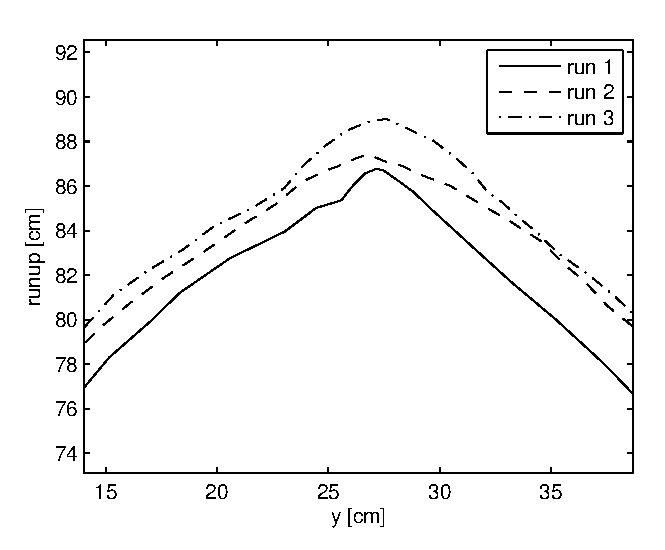
\includegraphics[width=0.95\textwidth]{Figures/runup10.eps}
                \caption{\textit{$A/H=0.0989$}}
                \label{fig:overflate_10}
        \end{subfigure}
         %add desired spacing between images, e. g. ~, \quad, \qquad, \hfill etc.
          %(or a blank line to force the subfigure onto a new line)
        \begin{subfigure}[H]{0.4\textwidth}
                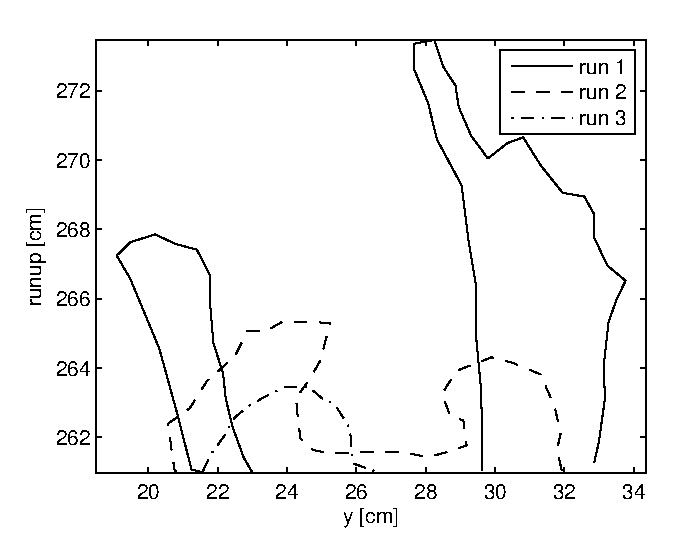
\includegraphics[width=0.95\textwidth]{Figures/runup50.eps}
                \caption{\textit{$A/H=0.4874$}}
                \label{fig:overflate_50}
        \end{subfigure}
}
        \caption{\textit{Shoreline shapes at max runup.}}
        \label{fig:max_runup}
\end{figure}

An estimate of the arrival time of the wave for FOV II, III and IV, were measured based on the intensity changes in images captured at each FOV.  Each image in each time series was compared to the initial image taken before the wave paddle starts. The image where the sum of light intensity differs more than a given threshold (1000) from the initial image, correspond to the time when the wave enters that FOV. The measured shoreline positions as a function time are presented in Figure \ref{fig:arr_tim}. The maximum error obtained for three different runs was 0.18\%. This indicate that the shoreline motion was repeatable for each of the FOV.
\begin{figure}
        \centering
        ~ %add desired spacing between images, e. g. ~, \quad, \qquad, \hfill etc.
          %(or a blank line to force the subfigure onto a new line)
                \includegraphics[scale=0.6]{./Figures/shoreline2015.eps}
                \caption{\textit{Shoreline position as a function of time for all cases. The first measurements correspond to the swash tongue arrival time for FOV I, II, III. The last measuring point for all cases correspond to measurement of maximum runup}}
              \label{fig:arr_tim}
      \end{figure}


\subsection{Velocity profiles from the swash zone}
\label{vel_pro}

Velocity profiles are extracted from the PIV data that are obtained from the four different FOV, approximately from 10cm to 120cm from the equilibrium shoreline. 
First, a comparison between computed BIM and measured PIV velocities for $A/H=0.989$ will be given for FOV I and II, (See Figure \ref{fig:BIM3_tim}). There is good agreement between measured and computed  velocity profiles. The computed velocities are larger in the front of the wave for both the FOVs. This complies with corresponding results in  \cite{pedersen2013runup} where the
delay of the experimental wave was linked to cappilary effects, while
an accumulative reduction of velocity, and hence runup height, was
related to the viscous bodary layers at the beach.  Hence, the BIM 
computation over-predicts the maximum runup as given in the previous section.\marginpar{Values ???}

\begin{figure}
        \centering
        ~ %add desired spacing between images, e. g. ~, \quad, \qquad, \hfill etc.
          %(or a blank line to force the subfigure onto a new line)
                \includegraphics[width=0.46\textwidth]{./Figures/BIM/case10_FOV3_PIV_BIM.eps}
                \includegraphics[width=0.46\textwidth]{./Figures/BIM/case10_FOV4_BIM_PIV.eps}
                \caption{\textit{\\ Left: Velocity profiles from FOV I x=8.7cm t=[7.48, 7.82, 8.15, 8.48, 8.81]s\\
                 \quad Right:  Velocity profiles from FOV II x=40.1cm t=[7.76, 8.10, 8.76, 9.10]s}}
              \label{fig:BIM3_tim}
      \end{figure}



 
%When a viscous fluid flows near a flat plate, a boundary layer can be obtain. Boundary layers are caused by viscous effect of the fluid and are also due to no-slip condition at the plate. Since there is a smooth transition from this trancient velocity area to the area of constant velocity, there is no defined line between boundary layer and the outer flow, but often is the boundary layer described as the area from the plate to the streamline where  $u =0.99U$.

 %Velocity profiles from the swash zone,  during flow reversal will be presented from FOV I,II and III. In addition, will the results be compared with a BIM boundary layer solution for the smallest waves, $A/H=0.0989$. 


%Underneath the solitary waves generated in this investigation, a boundary layer were obtained close to the beach (Figure \ref{fig:PIV_FOV4}). This can be interpreted that viscous effects are of great importance in analysis of swash tongues. Especially since the boundary layer occupying a large portion of the swash tongue thickness. The event of a swash tongue moving with a velocity U upward a beach can be compared to the problem of accelerating an infinite long plate from rest to a constant velocity U with a viscous fluid on top (Stokes first problem). Dimensional analysis gives us the relationship $\delta \approx \sqrt{\nu t}$.
%By introducing dimensional analysis to this problem an approximation to the boundary layer thickness can be found. If a flat plate suddenly accelerate to a velocity U, it will take some time for the motion to diffuse into the fluid on top. As a result the length of the area affected by the plate change in velocity (boundary layer thickness $\delta$) must be dependent on the time since the incident.The viscosity of the fluid will also affect how large the boundary layer will become.



%Velocity profiles for non-breaking solitary waves are studied experimentally by \cite{pedersen2013runup}.Their measurements revealed that the velocity profiles obtained close to the still water shoreline, had a viscous boundary layer close to the beach, and a uniform velocity U outside the boundary layer (the outer flow). 


FOV II is located approximately 40cm from the origin, and velocity 
profiles obtained from this FOV are shown in Figure \ref{fig:PIV_FOV4}.
For $A/H=0.1981$ the particle density was too sparse close to the surface, which led to spurious vacillations in the velocity profiles near  $z\approx1$. 
%Hit Geir: 1/3 10.25
 An outer flow seems to be constant for both non-breaking and breaking waves. The event of a swash tongue moving with a constant velocity U upward a beach, can be compared to the problem of accelerating an infinite long plate from rest to a constant velocity U with a viscous fluid on top, Stokes first problem \citep{white2006viscous}. Dimensional analysis will then give us a relationship between the boundary layer thickness $\delta $ and the viscosity $\nu$ and the time $t$,  $\delta \approx \sqrt{\nu t}$.  This implies that the boundary layer will grow with time, and this seems to be the case for the small non-breaking waves with amplitude  $A/H=0.0989$ (Figure \ref{fig:BIM3_tim}). However, for the strong plunging breakers the boundary layer decreases with time. This implies that the motion is more  irregular than for the non-breaking waves. %In addition, is the boundary layer thicker for the breaking waves. 
% For $A/H=0.2958$ to $A/H=0.4874$ the outer flow seems to start at higher values of z than for the non-breaking cases, this may imply that viscous effects has a larger influence on the breaking cases. For $A/H=0.0989$ to $A/H=0.1981$ the flow can be divided into three regions, the upper region (outer flow) where $\frac{du}{dz}=0$, the middle region where $\frac{du}{dz}>0$ and the region closest to the beach wall, where $\frac{du}{dz}<0$. 
% For breaking cases $A/H=0.2958-0.4874$, it seemed that the region closest to the wall where $\frac{du}{dz}<0$ is almost non existent for the velocity profiles obtained before flow reversal. This can be interpreted as irregular motion. The section where $\frac{du}{dz}<0$, reoccurred for the velocity profiles obtained after flow reversal for cases  $A/H=0.2958-0.4874$. This indicated that the deceleration of the field makes the motion more regular.

\begin{figure}[]
\centering
\makebox[\linewidth][c]{%
\begin{subfigure}[b]{.3\textwidth}
\centering
\includegraphics[width=.95\textwidth]{./Figures/BIM/profil10_feb.eps}
\caption{\textit{$A/H=0.0989$}}
\end{subfigure}%
\begin{subfigure}[b]{.3\textwidth}
\centering
\includegraphics[width=.95\textwidth]{./Figures/BIM/profil12_feb.eps}
\caption{\textit{$A/H=0.1191$}} 
\end{subfigure}%
\begin{subfigure}[b]{.3\textwidth}
\centering
\includegraphics[width=.95\textwidth]{./Figures/BIM/profil20_feb.eps}
\caption{\textit{$A/H=0.1981$}}
\end{subfigure}%
}
\makebox[\linewidth][c]{%
\begin{subfigure}[b]{.3\textwidth}
\centering
\includegraphics[width=.95\textwidth]{./Figures/FOV_4/case30_sept2015.eps}
\caption{\textit{$A/H=0.2958$}}
\end{subfigure}%
\begin{subfigure}[b]{.3\textwidth}
\centering
\includegraphics[width=.95\textwidth]{./Figures/FOV_4/case40_sept2015.eps}
\caption{\textit{$A/H=0.3939$}}
\end{subfigure}%
\begin{subfigure}[b]{.3\textwidth}
\centering
\includegraphics[width=.95\textwidth]{./Figures/FOV_4/case50_sept2015.eps}
\caption{\textit{$A/H=0.4874$}}
\end{subfigure}%
}
\caption{ \textit{FOV II, mean velocity profiles before  and after the outer flow reverses ($\triangle$,$\square$). Colors: blue, cyan, green and red correspond to run 1,2,3 and BIM respectively.  $x=40.11cm$. } }
\label{fig:PIV_FOV4}
\end{figure}
 FOV III is located about 80cm from origo along the beach. For $A/H=0.0989$ and $A/H=0.1191$, the swash tongues were too thin, and particles within the tongue were impossible to detect. Consequently, only $A/H=0.1981-0.4874$ will be presented for this FOV. None of the cases had an outer flow with constant velocity at times close to outer flow reversal (Figure \ref{fig:PIV_FOV5}). This indicates that the motion was more irregular for this FOV than for FOV II.
 \begin{figure}[]
\centering
\makebox[\linewidth][c]{%
\begin{subfigure}[b]{.3\textwidth}
\centering
\includegraphics[width=.95\textwidth]{./Figures/FOV_5/PIV_FOV5_case20.eps}
\caption{$A/H=0.1981$}
\end{subfigure}%
\begin{subfigure}[b]{.3\textwidth}
\centering
\includegraphics[width=.95\textwidth]{./Figures/FOV_5/PIV_FOV5_case30.eps}
\caption{$A/H=0.2958$}
\end{subfigure}%
}
\makebox[\linewidth][c]{%
\begin{subfigure}[b]{.3\textwidth}
\centering
\includegraphics[width=.95\textwidth]{./Figures/FOV_5/PIV_FOV5_case40.eps}
\caption{$A/H=0.3939$}
\end{subfigure}%
\begin{subfigure}[b]{.3\textwidth}
\centering
\includegraphics[width=.95\textwidth]{./Figures/FOV_5/PIV_FOV5_case50.eps}
\caption{$A/H=0.4874$}
\end{subfigure}%
}
\caption{ \textit{FOV III, mean velocity profiles before and after the outer flow reverses ($\triangle$,$\square$). Colors: blue, cyan and green correspond to run 1,2 and 3. 
$x=81.40cm$} }
\label{fig:PIV_FOV5}
\end{figure}

 FOV IV is located about 120cm from where the still water reaches the beach. At this FOV, only $A/H=0.2958-0.4874$ will be presented due to the thin swash tongue for the other waves. Velocity profiles are given in Figure \ref{fig:PIV_FOV6}. The velocity was less repeatable at this location than for the other FOVs. The velocity profiles seemed to be more irregular, especially for $A/H=0.4874$, where the average velocity profile obtained before flow reversal resembles the parbolic velocity profiles from fully developed turbulent channel flow, as described in \cite{white2006viscous}. %For laminar channel flow the velocity profiles has parabolic shape, and as the reynold number increases to fully developed turbulent channel flow, the velocity profiles has a larger area in middle of the channel where the velocity is constant. The velocity decays closer to the walls for turbulent regimes than for the laminar flow regimes. The mean velocity profile obtained for $A/H=0.4874$ has a shape that resembles the time average velocity profile for turbulent channel flow in addition to a frequent fluctuating velocity around this mean.

%The shape of the velocity profiles seems to differ more from the shape observed for the non-breaking solitary waves in \citep{pedersen2013runup} as we move further up the beach. In addition, it seems like stronger breakers differs more from the non-breaking shape, than the small breakers. Overall, the velocities before and after flow reversal, seemed to become more irregular as the waves washes up the beach.  
\begin{figure}[]
\centering
\makebox[\linewidth][c]{%
\begin{subfigure}[b]{.3\textwidth}
\centering
\includegraphics[width=.95\textwidth]{./Figures/FOV_6/PIV_FOV6_case30.eps}
\caption{\textit{$A/H=0.2958$}}
\end{subfigure}%
\begin{subfigure}[b]{.3\textwidth}
\centering
\includegraphics[width=.95\textwidth]{./Figures/FOV_6/PIV_FOV6_case40.eps}
\caption{\textit{$A/H=0.3939$}}
\end{subfigure}%
\begin{subfigure}[b]{.3\textwidth}
\centering
\includegraphics[width=.95\textwidth]{./Figures/FOV_6/PIV_FOV6_case50.eps}
\caption{\textit{$A/H=0.4874$}}
\end{subfigure}%
}
\caption{\textit{FOV IV, mean velocity profiles before and after the outer flow reverses ($\triangle$,$\square$). Colors: blue, cyan and green correspond to run 1,2 and 3. 
$x=121.25cm$} }
\label{fig:PIV_FOV6}
\end{figure}
\begin{figure}[]
        \centering
        ~ %add desired spacing between images, e. g. ~, \quad, \qquad, \hfill etc.
          %(or a blank line to force the subfigure onto a new line)
                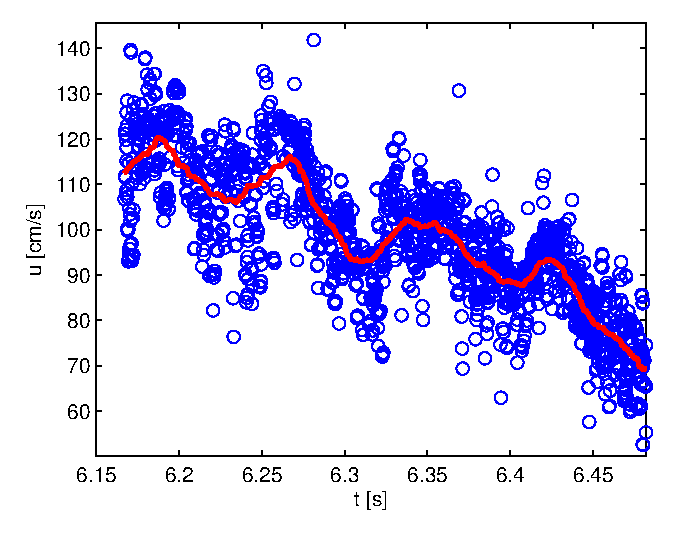
\includegraphics[scale=0.6]{./Figures/tid_case50_run2.eps}
                \caption{\textit{FOV III Collection of velocities of particles within a distance of 0.05cm from the point(x,z)=(120,0.3)cm. The data is collected from  $A/H=0.4874$, run 2. Blue circles: Raw data points. Red line: 2 order interpolation with 40 evaluation points}}
                \label{fig:wave_in_time}
        \end{figure}      
         
Inspection of movies of the front of the swash tongue from FOV IV (furthest up the beach) shows that a systematic swirling effect were present in the front of the swash tongue.  Particle Tracking Velocimetry (PTV) have been utilized to investigate this phenomenon. Figure \ref{fig:wave_in_time} shows how the velocities vary at one spot in fluid as a function of time. The velocities seem to oscillate, in addition to a linear decaying trend. The red line represents an interpolation of all the data, where 40 points are considered at each evaluation point. This indicates that there is a systematic velocity field in the front of the swash tongue. 


 
 \subsection{Bubble investigation}
 \label{bub_inv}
 For all the plunger breakers, the plunge encapsulated air, resulting in one large air bubble. As the waves propagated upward the beach, this large air bubble divided into smaller air bubbles, which again divided into even smaller air bubbles. Before reaching maximum runup,  all the air bubbles had risen to the surface, for all waves. The images captured with the large FOV A provides some information about this air bubble formation, (see Figure \ref{fig:bubble_30} and \ref{fig:bubble_50}). To enhance the shape of the bubbles the gradient magnitude image is represented. The shape of main bubble seems to be oval with a thin tongue in the front, for $A/H=0.2958$. The shape of the main air bubble seems to vary more for $A/H=0.4874$, especially for run2, where the large air bubble can't be found in the image. The length of the main bubble for three different runs is given in Table \ref{tab:b_case30}. It is clear that images from the three different runs for $A/H=0.2958$ is more similar than for $A/H=0.4874$. This supports the hypothesis that irregularity increases as normalized amplitude of the waves increases.

The air bubble velocity in the direction along the beach is given in Table \ref{vel_bubb}. The largest velocities were obtained in the front of the bubbles, and may explain the shape of the thin tongue in the front of the air bubble observed for $A/H=0.2958$. The bubble findings indicates that the motion becomes more irregular as the amplitude of the waves increases.
\begin{figure}[]
\centering
\includegraphics[width=0.7\textwidth]{./Figures/BUBBLE/bubble_30_run1.eps}
\includegraphics[width=0.7\textwidth]{./Figures/BUBBLE/bubble_30_run2.eps}
\includegraphics[width=0.7\textwidth]{./Figures/BUBBLE/bubble_30_run3.eps}
%http://commons.wikimedia.org/wiki/File:Breaking_wave_types.gif
\caption{\textit{$A/H=0.2958$, run 1,2 and 3. t=6.06s}}
\label{fig:bubble_30}
\end{figure}

\begin{figure}[]
\centering
\includegraphics[width=0.6\textwidth]{./Figures/BUBBLE/bubble_50_run1.eps}
\includegraphics[width=0.6\textwidth]{./Figures/BUBBLE/bubble_50_run2.eps}
\includegraphics[width=0.6\textwidth]{./Figures/BUBBLE/bubble_50_run3.eps}
%http://commons.wikimedia.org/wiki/File:Breaking_wave_types.gif
\caption{\textit{$A/H=0.4874$, run 1,2 and 3. t=5.54s}}
\label{fig:bubble_50}
\end{figure} 


\begin{table}[]
\centering
\caption{\textit{ Size of the main bubble measured at t=6.06s for case 30, and t=5.54s for case 50}}
\label{my-label}
\begin{tabular}{|c|c|c|c|}
\hline
\textbf{Main bubble size }              & \textbf{Run 1 {[}cm{]}} & \textbf{Run 2 {[}cm{]}} & \textbf{Run 3 {[}cm{]}} \\ \hline
$A/H=0.2958$:  & 8.00     & 8.94     & 7.90     \\ \hline
$A/H=0.4874$: & 9.24     &      & 8.17     \\ \hline
\end{tabular}
\label{tab:b_case30}
\end{table}
 
%\begin{table}[]
%\centering
%\caption{Size of the main bubble measured at t=5.54s for case 50}
%\label{my-label}
%\begin{tabular}{|c|c|c|c|}
%\hline
%\textbf{Run}              & \textbf{1} & \textbf{2} & \textbf{3} \\ \hline
%Main bubble size {[}cm{]} & 9.2426     & 7.5314     & 8.2136     \\ \hline
%\end{tabular}
%\label{tab:b_case50}
%\end{table}
 
\begin{table}[]
\centering
\caption{\textit{ Velocities along the beach for the main air bubble.  t=6.06s for case 30, and t=5.54s for case 50}}
\label{vel_bubb}
\begin{tabular}{llll}
\hline
{\bf $A/H=0.2958$}                    & Run 1 & Run 2 & Run 3 \\ \hline
Front velocity {[}m/s{]}  & 2.05  & 2.20  & 2.48  \\
Tail velocity {[}m/s{]}  & 2.10  & 2.05  & 2.23  \\ \hline
{\bf $A/H=0.4874$}                    &       &       &       \\ \hline
Front velocity {[}m/s{]}  & 3.26  &   & 2.01  \\
Tail velocity {[}m/s{]}   & 1.58  &   & 2.23 
\end{tabular}
\end{table} 
 
 
%\begin{table}[h]
%\center
%\begin{tabular}{|l|l|l|l|}
%\hline
%{\bf $A/H=0.2958$}            & {\bf Run 1} & {\bf Run 2} & {\bf Run 3} \\ \hline
%Front velocity {[}m/s{]} & 2.05        & 2.20        & 2.48        \\ \hline
%Tail velocity {[}m/s{]}  & 2.10        & 2.05        & 2.23        \\ \hline
%{\bf Case 50}            & {\bf Run 1} & {\bf Run 2} & {\bf Run 3} \\ \hline
%Front velocity {[}m/s{]} & 3.26       &2.58        & 2.01        \\ \hline
%Tail velocity {[}m/s{]}  & 1.58         & 2.40        & 2.23        \\ \hline
%\end{tabular}
%\caption{My caption}
%\label{my-label}
%\end{table} 
 
%\begin{table}[h]
%\centering
%\begin{tabular}{|l|l|l|l|}
%\hline
%{\bf Case 50}            & {\bf Run 1} & {\bf Run 2} & {\bf Run 3} \\ \hline
%Front velocity {[}m/s{]} & 3.26       &2.58        & 2.01        \\ \hline
%Tail velocity {[}m/s{]}  & 1.58         & 2.40        & 2.23        \\ \hline
%\end{tabular}
%\caption{My caption}
%\label{my-label}
%\end{table} 
 
\section{Discussion}
\label{con_rem}

%The smallest cases with $A/H \approx 0.10, 0.12 $ did not break while propagating on a beach with inclination $5.1^\circ$ . All the other waves developed into plunging breakers. Surface elevation of the incident waves were measured with ultrasonic gauges, and coincided with theory from \cite{tanaka1986stability}. PIV  were performed on images captured from three different FOVs. The FOVs were located from 40cm to 120cm from where the still water level intersected with the beach. 


The experimental result from  the non-breaking  waves generated in this study coincide with the numerical result from BIM model. Both, the surface elevation and velocities seems to agree with numerical result. However, deviations between the computed and the measured maximum runup  was observed for the smallest waves. Also the BIM model over predict the velocity in front of the wave. Discrepancies between computation and measurement may be due to viscosity effect in the thin swash tongue, but may also be caused by bending effects of the beach. The beach bended due to its own weight and an additional bending was also observed due to wave load. 

The measurement of the breaking waves showed that the fluid motion becomes more irregular and less repeatable as we move further up the beach. In addition, the motion seemed to be more irregular for the waves with the stronger plunger breakers than for those with smaller amplitude. The maximum runup was repeatable in both time and height, but large variation of the cross shore profiles was obtained for the breaking waves. The results from the bubble investigation showed that the air bubble seemed to be repeatable in shape for the waves with amplitude $A/H=0.2958$ but not for waves with amplitude  $A/H=48.74$. Overall, irregular motion seems to increase with larger breaking waves and as the waves propagate upwards the beach.  

\section*{Acknowledgment}

This work was funded by the Research Council of Norway through the research project DOMT - Developments in Optical Measurement Technologies (project number 231491).
 \bibliography{bibliography}
\bibliographystyle{pjgsm}


\end{document}

